%%%%%%%%%%%%%%%%%%%%%%%%%%%%%%%%%%%%%%%%%%%%%%%%%%%%%%%%%%%%%%%%%%%%%%%%%%%%%%%%
% VocalCoach — Final Project Report (TISMIR template)
%%%%%%%%%%%%%%%%%%%%%%%%%%%%%%%%%%%%%%%%%%%%%%%%%%%%%%%%%%%%%%%%%%%%%%%%%%%%%%%%

\documentclass{article}

\usepackage[utf8]{inputenc}
\usepackage{tismir}
\usepackage{amsmath}
\usepackage{hyperref}
\usepackage{url}
\usepackage{graphicx}
\usepackage{booktabs}
\usepackage{tabularx}

%%%%%%%%%%%%%%%%%%%%%%%%%%%%%%%%%%%%%%%%%%%%%%%%%%%%%%%%%%%%%%%%%%%%%%%%%%%%%%%%
% Title and Author information
%%%%%%%%%%%%%%%%%%%%%%%%%%%%%%%%%%%%%%%%%%%%%%%%%%%%%%%%%%%%%%%%%%%%%%%%%%%%%%%%

\title{VocalCoach: A Single-Backbone Multi-Task Model for\\
Robust Offline Singing Analysis and Coaching}

\author{Rajat Sharma\thanks{MS in Computer Engineering, Drexel University}}

\date{}

\type{research}

\authorref{Sharma,~R.}
\authorshort{Sharma}
\titleshort{VocalCoach: Single-Backbone Singing Analysis}

%%%%%%%%%%%%%%%%%%%%%%%%%%%%%%%%%%%%%%%%%%%%%%%%%%%%%%%%%%%%%%%%%%%%%%%%%%%%%%%%
\begin{document}

\twocolumn[{%
%
\maketitleblock
%
\begin{abstract}
VocalCoach is an offline singing-analysis system that turns one vocal recording
into structured coaching feedback. From a single forward pass of a 7.8M-parameter
temporal-convolutional backbone, it produces pitch (F0), voice activity, singing
technique, note onsets/offsets, and a quality score, rendered as a browser coaching
report. The central problem is robustness: models trained on clean studio audio
degrade on real-world recordings made with consumer microphones. On-the-fly gain and
spectral-tilt augmentation help close that gap, lifting out-of-distribution
voiced-detection rate from $\sim$53\% to 68\% while holding pitch accuracy at 99\%
in-distribution (72\% out-of-distribution). Technique reaches 80.8\% clip accuracy
(matching published VocalSet state-of-the-art) and the note head reaches 0.81
onset/offset F1. The key result is methodological: each capability is best served by
a \emph{VAD-preserving probe} on a shared, augmentation-hardened backbone rather than
a single jointly-trained model. Several plausible additions (a falsetto specialist, a
nine-dimension quality head) were measured, found not to separate, and dropped.
\end{abstract}
%
\begin{keywords}
singing voice analysis, multi-task learning, pitch estimation, singing technique,
note transcription, domain robustness
\end{keywords}
}]
\saythanks{}

%%%%%%%%%%%%%%%%%%%%%%%%%%%%%%%%%%%%%%%%%%%%%%%%%%%%%%%%%%%%%%%%%%%%%%%%%%%%%%%%
% 1. Goal & Motivation
%%%%%%%%%%%%%%%%%%%%%%%%%%%%%%%%%%%%%%%%%%%%%%%%%%%%%%%%%%%%%%%%%%%%%%%%%%%%%%%%
\section{Goal and Motivation}\label{sec:goal}

\textbf{Vocal coach.} VocalCoach is an automated singing tutor: a singer uploads
a recording and receives the feedback a human vocal coach would give --- what pitch
was sung, whether notes were stable, which techniques were used (vibrato, breathiness,
belting), where the phrases were, and an overall quality assessment --- with an
optional reference recording to compare against.

\textbf{Target user and problem.} The target user is an amateur or a journeyman singer
practising alone, without access to a coach. The concrete problem is that existing
tools are either pitch-only tuners that say nothing about technique or musical quality,
or cloud services that assume studio-quality input and fail on real-world conditions. 
Real practice audio can be quiet, noisy, and
affected by inexpensive
microphones --- exactly the scenario where research models, trained on clean audio,
break down.

\textbf{System goal.} \emph{Produce a complete, technique-aware coaching report from a
single real-world singing clip, robustly enough to work on amateur recordings, in one
offline pass of one shared model.}

%%%%%%%%%%%%%%%%%%%%%%%%%%%%%%%%%%%%%%%%%%%%%%%%%%%%%%%%%%%%%%%%%%%%%%%%%%%%%%%%
% 2. Related Work
%%%%%%%%%%%%%%%%%%%%%%%%%%%%%%%%%%%%%%%%%%%%%%%%%%%%%%%%%%%%%%%%%%%%%%%%%%%%%%%%
\section{Related Work}\label{sec:related}

Singing analysis spans several sub-problems usually solved separately; our contribution
is unifying them on one robust backbone and being disciplined about which capabilities
hold up.

\textbf{Pitch estimation.} CREPE~\cite{Kim2018_CREPE_ICASSP} and
RMVPE~\cite{Wei2023_RMVPE_INTERSPEECH} frame F0 estimation as classification over a
binned posteriorgram. We adopt this formulation (360 bins, 20-cent resolution) and use
RMVPE to generate training labels, but unlike these single-task models we share the
pitch representation with four other heads and add an offline Viterbi decode for clean
F0 tracks.

\textbf{Singing-technique classification.} Recent classifiers on
VocalSet~\citep{Wilkins2018_VocalSet_ISMIR} report $\sim$80\% clip accuracy on its
technique classes. We match this (80.8\%) but show that the commonly-paired GTSinger
falsetto data~\citep{Zhang2024_GTSinger_NEURIPS} does not add a usable fifth class once
measured properly.

\textbf{Note transcription.} Frame-level onset/offset
detection~\citep{Hawthorne2018_OnsetsFrames_ISMIR} combined with a pitch posteriorgram
yields discrete notes. Our note head follows this design; our finding is that the
\emph{pitch-at-note} ceiling is set by the posteriorgram's octave errors, not the onset
detector.

\textbf{Singing quality.} SingMOS~\citep{SingMOS2024} provides scalar mean-opinion
scores. We distil a scalar quality head from it with a contrastive pro-versus-amateur
ranking term, and show that multi-dimensional expert ratings we examined are too
inter-correlated to learn as independent axes.

Our augmentation pipeline follows SpecAugment~\citep{Park2019_SpecAugment_INTERSPEECH}
and extends it with gain and spectral-tilt perturbations targeting the loudness and
microphone-colour gap specific to amateur recording setups.

%%%%%%%%%%%%%%%%%%%%%%%%%%%%%%%%%%%%%%%%%%%%%%%%%%%%%%%%%%%%%%%%%%%%%%%%%%%%%%%%
% 3. System Overview
%%%%%%%%%%%%%%%%%%%%%%%%%%%%%%%%%%%%%%%%%%%%%%%%%%%%%%%%%%%%%%%%%%%%%%%%%%%%%%%%
\section{System Overview}\label{sec:overview}

A single log-mel input (40 bands, 16\,kHz) passes through one shared backbone --- 8
dilated temporal-convolution blocks plus 4 self-attention layers (hidden $=256$) ---
to produce frame features of shape $(B, T, 256)$. From these, five lightweight heads
read off all outputs in one forward pass, as summarised in
Table~\ref{tab:heads} and Figure~\ref{fig:arch}.

Four of the heads are per-frame, but the quality head
\emph{mean-pools the frame features over time first} ($\mathbf{x}.\mathrm{mean}(\dim=1)$)
and emits a single clip-level score --- it does not see per-frame features. The browser
UI consumes this report to draw the waveform with voice activity, the log-mel
spectrogram, the pitch posteriorgram, a note timeline, a per-phrase breakdown (with
clip-segment playback), the detected technique, and the overall score. An optional
reference recording is analysed in the same pass for an A/B comparison with synced
playback.

\begin{table}[htbp]
\centering
\begin{tabularx}{\columnwidth}{l l X}
\toprule
\bfseries Head & \bfseries Granularity & \bfseries Output \\
\midrule
Pitch       & per-frame  & 360-bin posteriorgram, F0 \\
VAD         & per-frame  & voiced / unvoiced \\
Technique   & per-frame  & 4 classes \\
Note        & per-frame  & onset/offset, MIDI \\
Quality     & clip-level & one 0--100 score \\
\bottomrule
\end{tabularx}
\caption{The five heads and their output granularity. Technique is per-frame in the
model but aggregated over voiced frames for display; quality is clip-level by
construction (time-pooled).}
\label{tab:heads}
\end{table}

\begin{figure}[htbp]
  \centering
  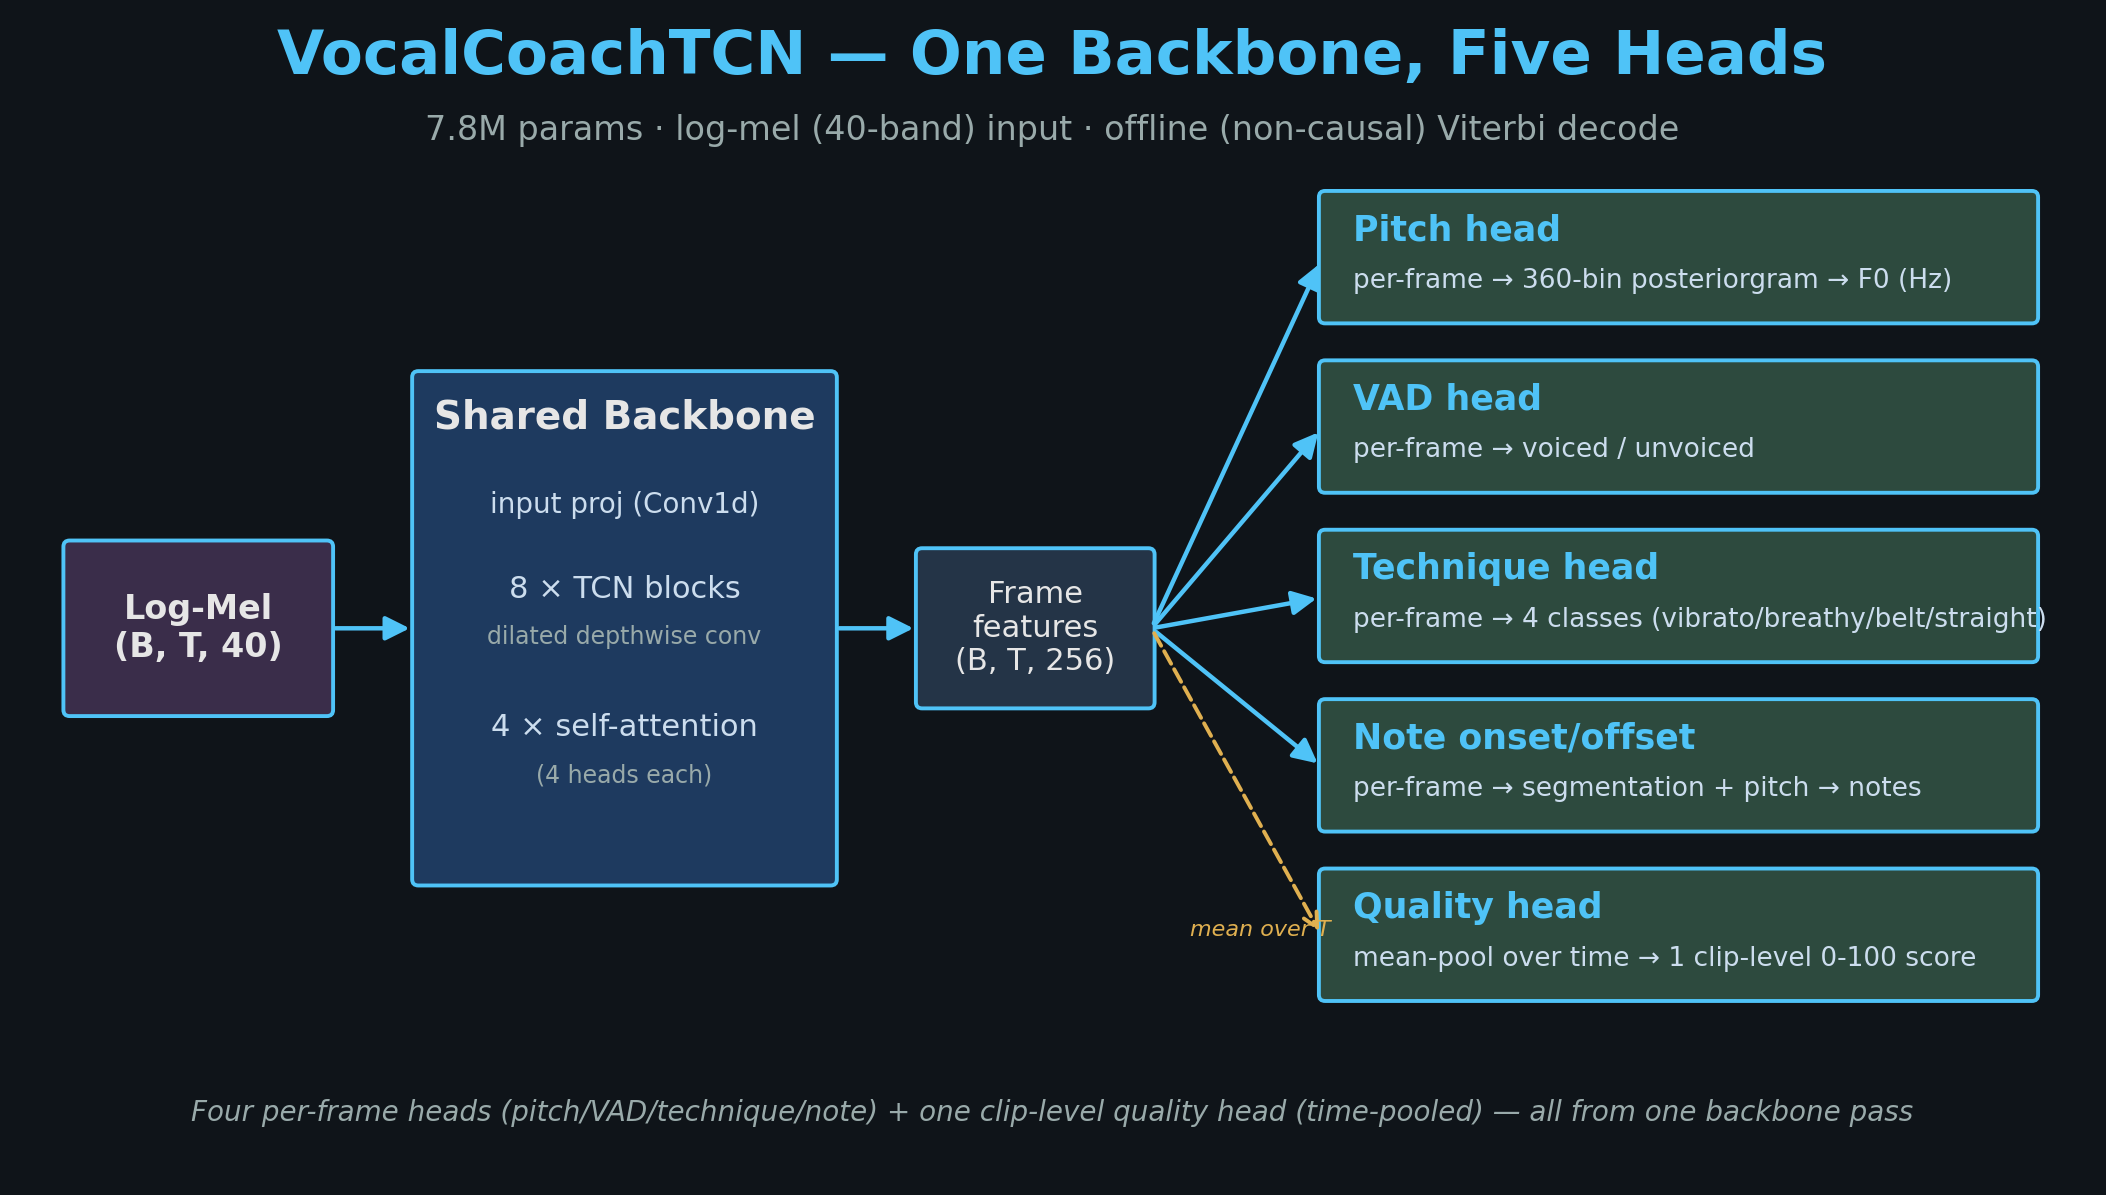
\includegraphics[width=\columnwidth]{architecture}
  \caption{VocalCoachTCN: one shared backbone feeds four per-frame heads
  (pitch, VAD, technique, note) and one clip-level quality head that mean-pools the
  frame features over time.}
  \label{fig:arch}
\end{figure}

\subsection{Demonstration}\label{sec:demo}

Figures~\ref{fig:ui-main} and~\ref{fig:ui-phrases} show the running system on a
real held-out clip (Vocadito). These are qualitative illustrations of the interface
and the coaching output, not quantitative evidence; the measured results are reported
in Section~\ref{sec:eval}. Figure~\ref{fig:ui-main} shows the top-level analysis ---
overall score, waveform with voice activity, log-mel spectrogram, and pitch
posteriorgram --- while Figure~\ref{fig:ui-phrases} shows the per-phrase coaching
breakdown, where each detected phrase carries its note, dynamics, and a
technique-specific comment with an actionable suggestion.

\begin{figure}[htbp]
  \centering
  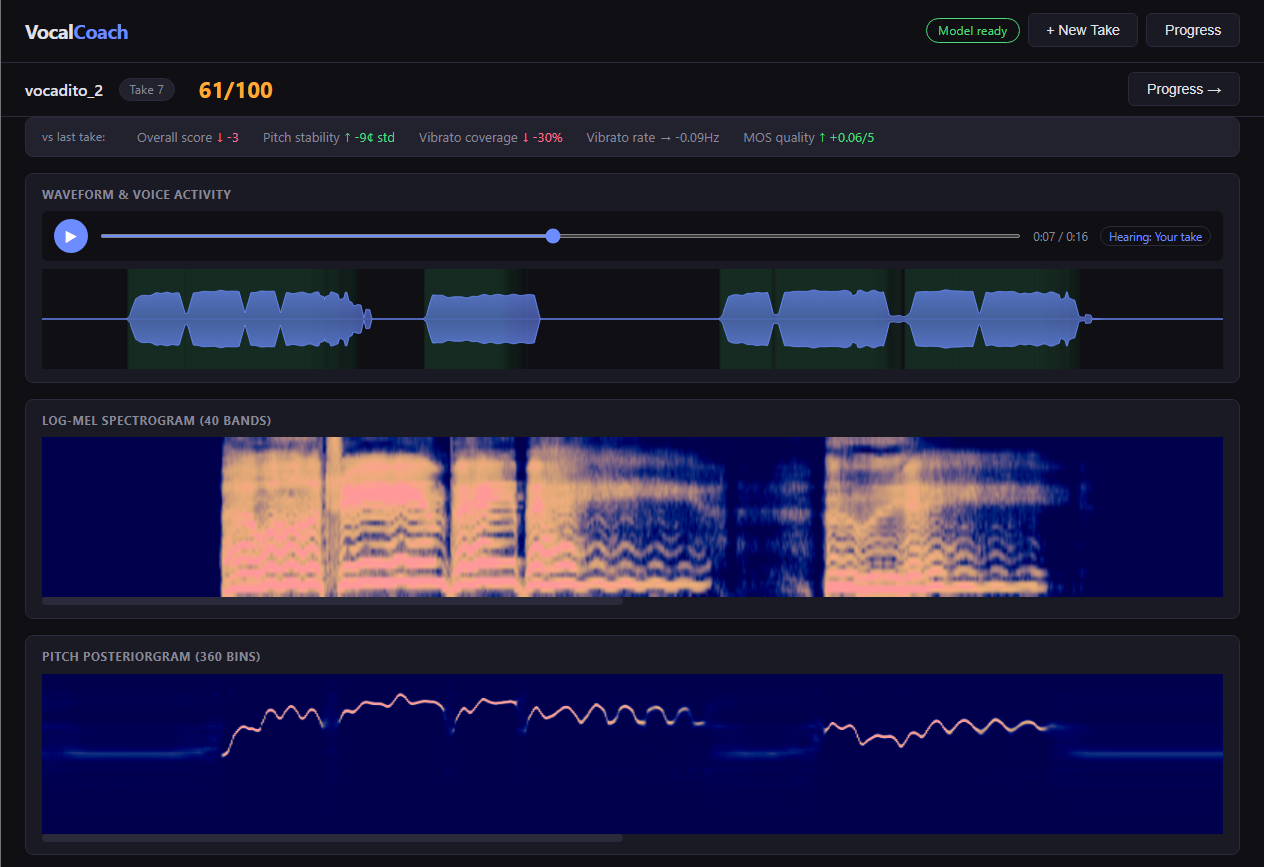
\includegraphics[width=\columnwidth]{ui_main}
  \caption{The analysis view on a real clip: overall score, waveform/voice activity,
  log-mel spectrogram, and pitch posteriorgram (Qualitative demonstration only).}
  \label{fig:ui-main}
\end{figure}

\begin{figure}[htbp]
  \centering
  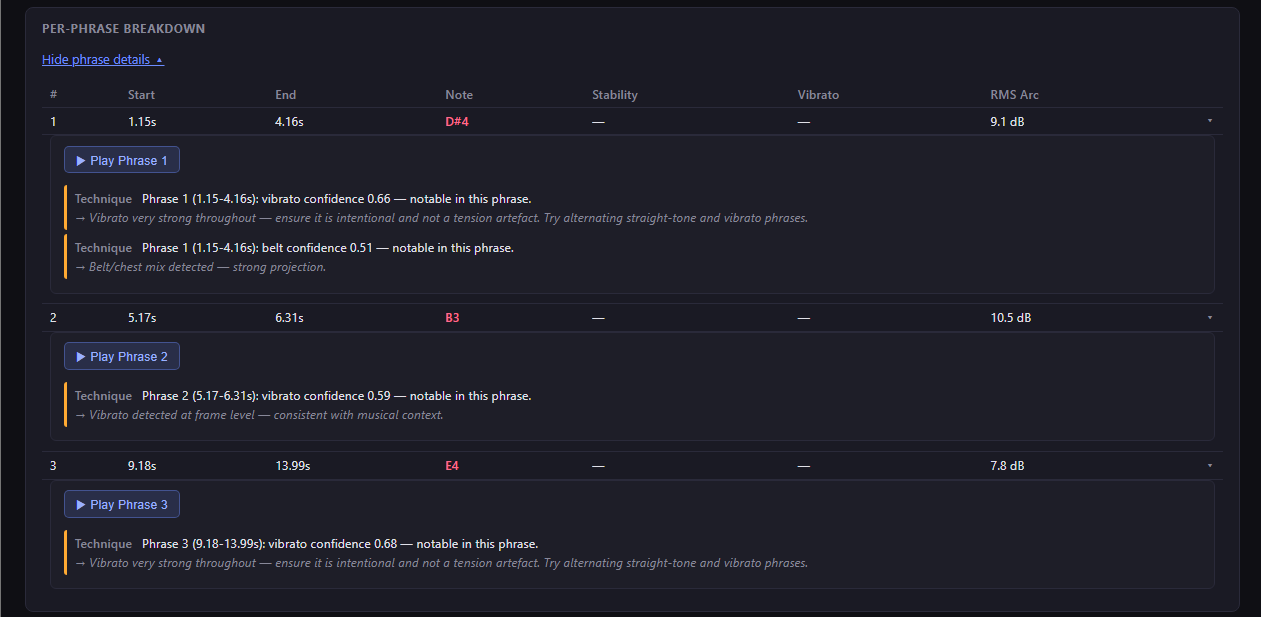
\includegraphics[width=\columnwidth]{ui_phrases}
  \caption{Per-phrase coaching breakdown: each phrase lists its note, RMS arc, and a
  technique-specific observation with an actionable tip, with per-phrase audio
  playback (Qualitative demonstration only).}
  \label{fig:ui-phrases}
\end{figure}

%%%%%%%%%%%%%%%%%%%%%%%%%%%%%%%%%%%%%%%%%%%%%%%%%%%%%%%%%%%%%%%%%%%%%%%%%%%%%%%%
% 4. Data
%%%%%%%%%%%%%%%%%%%%%%%%%%%%%%%%%%%%%%%%%%%%%%%%%%%%%%%%%%%%%%%%%%%%%%%%%%%%%%%%
\section{Data}\label{sec:data}

Each capability is supervised by the dataset best suited to it
(Table~\ref{tab:data}); all are public and linked rather than redistributed.

\begin{table}[htbp]
\centering
\begin{tabularx}{\columnwidth}{@{}l l X@{}}
\toprule
\bfseries Use & \bfseries Dataset & \bfseries Size \\
\midrule
Pitch / VAD & Merged P-VAD     & 51{,}627 clips, 126\,h \\
Technique   & VocalSet         & 824 clips \\
Note        & Annot.\ VocalSet & 824 clips, 4.5k notes \\
Quality     & SingMOS+pairs    & MOS, pro/amateur \\
OOD eval    & Vocadito         & 40 real recordings \\
\bottomrule
\end{tabularx}
\caption{Datasets, one per capability. Vocadito is held entirely out of training as
the out-of-distribution (OOD) generalisation test.}
\label{tab:data}
\end{table}

\textbf{Provenance and preprocessing.} All audio is resampled to 16\,kHz mono; features
are log-mel (40 bands) plus RMVPE-derived F0 targets binned to a 360-class
posteriorgram (20 cents/bin). Note MIDI labels are integer-quantised to the nearest
semitone.

\textbf{Augmentation (the core robustness lever).} All augmentation is applied
on-the-fly at train time (stored features stay clean), and all of it is
label-preserving: \emph{gain} (random $-40 \to 0$\,dB, simulating quiet recordings),
\emph{spectral-tilt} (random per-band EQ, simulating microphone/room colour),
\emph{noise mixing} (FSDNoise/MUSAN noise at random SNR), and SpecAugment time/frequency
masking. Pitch-shift and time-stretch are additionally available offline for technique
data, with labels re-derived.

\textbf{Limitations and bias.} (1) The technique and note corpora are VocalSet-only ---
Western, mostly classically-trained singers --- so technique predictions are biased
toward that style. (2) Note-pitch labels are semitone-quantised, so expressive
vibrato and portamento are inherently ambiguous against a $\pm$50-cent tolerance.
(3) The SingMOS scale is not calibrated to our user population, and the
multi-dimensional expert ratings we inspected are $\approx 0.95$ inter-correlated ---
they carry little independent signal.

%%%%%%%%%%%%%%%%%%%%%%%%%%%%%%%%%%%%%%%%%%%%%%%%%%%%%%%%%%%%%%%%%%%%%%%%%%%%%%%%
% 5. Model
%%%%%%%%%%%%%%%%%%%%%%%%%%%%%%%%%%%%%%%%%%%%%%%%%%%%%%%%%%%%%%%%%%%%%%%%%%%%%%%%
\section{Model}\label{sec:model}

\textbf{Architecture.} \texttt{VocalCoachTCN}, 7.8M parameters: an input projection
(Conv1d) feeds 8 dilated depthwise-separable TCN blocks (kernel 31, exponentially
increasing dilation for a wide receptive field well-matched to vibrato periodicity and
phrase length), then 4 multi-head self-attention layers (4 heads each), producing frame
features $(B, T, 256)$ and the five heads of Section~\ref{sec:overview}.

\textbf{Inputs and outputs.} Input $(B, T, 40)$ log-mel. Outputs: pitch $(B, T, 360)$,
VAD $(B, T, 1)$, technique $(B, T, 4)$, note onset/offset $(B, T, 1)$ each, and quality
$(B, 1)$. At inference the pitch posteriorgram is Viterbi-decoded with full-clip
context; notes are formed by peak-picking onsets/offsets and reading per-note MIDI from
the posteriorgram (octave-collapsed, confidence-weighted mean over the span).

\textbf{Design rationale.} We do \emph{not} jointly train one model on everything, and
we do \emph{not} fine-tune the whole backbone per task. Fine-tuning the backbone on
technique lifts technique average precision (0.70 $\to$ 0.93) but erodes the
loudness-robust VAD (clean voiced-detection rate 87\% $\to$ 63\%) --- the exact
robustness the augmentation bought. The resolution is a \emph{VAD-preserving probe}:
train an augmentation-hardened pitch/VAD/note backbone once (gain + spectral-tilt),
then attach each new head as a probe on the frozen (or differentially low-learning-rate)
backbone. This keeps OOD VDR intact while still reaching state-of-the-art technique
accuracy. The deployed system is therefore one backbone plus per-head probes, each
adding one forward pass.

\textbf{Training details.} Pitch is a VAD-masked binary cross-entropy over the
posteriorgram (Gaussian target, $\sigma = 0.8$ bins). Note onset/offset uses
positive-weighted BCE (weight 35) because boundaries are $\sim$2--3\% of frames and
unweighted BCE collapses to the majority class. A small
octave-confusion penalty on the pitch head was tried for the note head and found not
to help; the error is intrinsic (Section~\ref{sec:eval}).

%%%%%%%%%%%%%%%%%%%%%%%%%%%%%%%%%%%%%%%%%%%%%%%%%%%%%%%%%%%%%%%%%%%%%%%%%%%%%%%%
% 6. Evaluation
%%%%%%%%%%%%%%%%%%%%%%%%%%%%%%%%%%%%%%%%%%%%%%%%%%%%%%%%%%%%%%%%%%%%%%%%%%%%%%%%
\section{Evaluation}\label{sec:eval}

\textbf{Metrics and why they connect to the goal.} Because the goal is \emph{robust}
coaching on \emph{real} audio, the headline results are the in-distribution versus
out-of-distribution (Vocadito, 40 recordings never seen in training). Per head: pitch
uses raw pitch accuracy (RPA, $\pm$50 cents) --- does the user see the right pitch?;
VAD uses voiced-detection rate (VDR) and voicing F1 (vF1), the hardest part on quiet
real audio and what the augmentation targets; technique uses clip accuracy (argmax,
matching the SOTA metric) and per-class F1 / macro AP; note uses onset/offset F1
(mir\_eval, $\pm$50\,ms) and note-with-pitch F1 (onset $\pm$50\,ms \emph{and} pitch
$\pm$50 cents), separating timing from pitch-at-note; quality uses Pearson/Spearman
correlation with MOS and mean absolute error, because the deployed score is the
absolute head output (the ranking head is a training diagnostic, not read at
inference).

\textbf{Headline results} (deployed checkpoints) are in Table~\ref{tab:results}.
Per-technique F1 on VocalSet is vibrato 0.94, breathy 0.84, belt 0.79, straight 0.78
(macro AP 0.87): the acoustically most distinctive techniques are detected most
reliably.

\begin{table}[htbp]
\centering
\begin{tabular}{llcc}
\toprule
\bfseries Head & \bfseries Metric & \bfseries In-dist & \bfseries OOD \\
\midrule
Pitch     & RPA               & 99\%   & 72\% \\
VAD       & VDR               & 88\%   & 68\% \\
VAD       & vF1               & 92\%   & 75\% \\
Technique & clip accuracy     & 80.8\% & --- \\
Note      & onset/offset F1   & 0.81   & --- \\
Note      & note-with-pitch F1& 0.53   & --- \\
Quality   & Pearson $r$ (MOS) & 0.54   & --- \\
\bottomrule
\end{tabular}
\caption{Headline results for the deployed checkpoints. OOD = Vocadito. Pitch and VAD
are reported both in-distribution and OOD; the other heads have no OOD test set.}
\label{tab:results}
\end{table}

\textbf{Discussion.} The augmentation result is the clearest win
(Figure~\ref{fig:pitchvad}): gain and spectral-tilt lifted OOD VDR from a $\sim$53\%
baseline to 68\% without hurting in-distribution (88\% VDR, 99\% RPA). RPA barely moves
OOD (99 $\to$ 72\%), confirming the residual gap is voicing, not pitch. Technique
matches published SOTA. For notes, timing is strong (0.81) but pitch-at-note plateaus
at $\sim$0.53: across 27 tuning runs it never escaped a 0.51--0.53 band. We traced this
to the backbone posteriorgram --- frame-level RPA is 94\% and unbiased, but $\sim$18--20\%
of notes carry a full-semitone octave/harmonic error that no span aggregation removes.
An inference-side fix (octave-collapse plus confidence-weighted mean) moved the number
from 0.50 to 0.53; the rest is intrinsic. Quality at Pearson 0.54 is a genuine if
modest correlation with MOS, and the light pro/amateur ranking term \emph{improved} the
absolute score (0.40 $\to$ 0.54) rather than fighting it.

\begin{figure}[htbp]
  \centering
  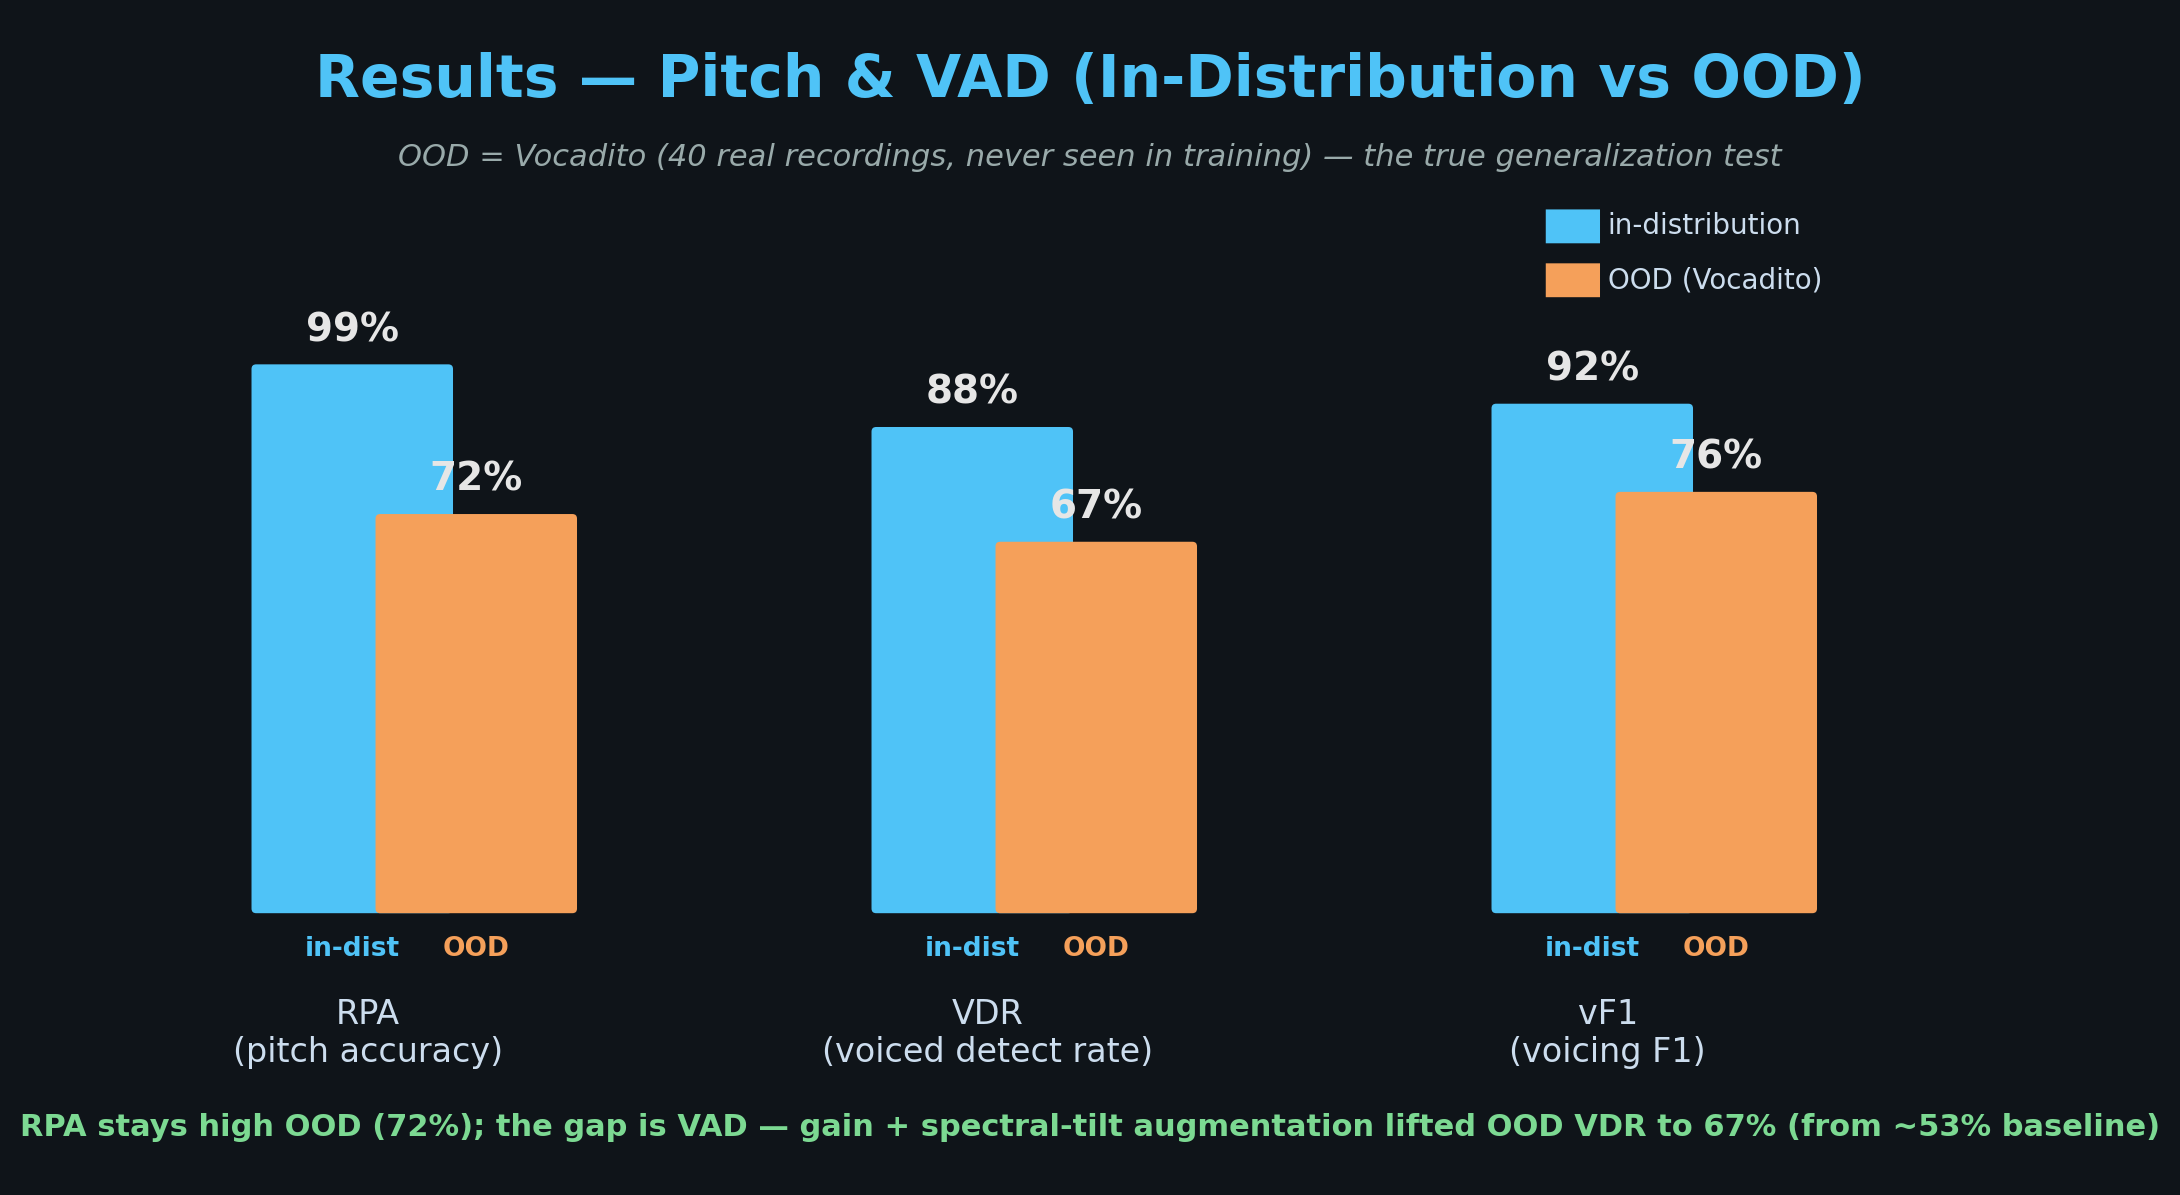
\includegraphics[width=\columnwidth]{results_pitchvad}
  \caption{Pitch and VAD, in-distribution versus OOD (Vocadito). Pitch accuracy holds
  up OOD; gain and spectral-tilt augmentation closed most of the voicing gap.}
  \label{fig:pitchvad}
\end{figure}

\textbf{Two negative results.} First, a GTSinger falsetto specialist
was trained to add a fifth technique class. On its own labelled test set it output
$\sim$0.70 falsetto probability on \emph{both} falsetto (0.704) and non-falsetto (0.679)
clips --- a 0.025 separation. No threshold distinguishes them; the apparently high F1
was the 71\% base rate. We dropped it and ship four trustworthy classes. Second, a
nine-dimension expert quality head could not learn independent dimensions because the
labels are $\approx 0.95$ inter-correlated, only 132 clips, and on a different (1--10)
scale; it also corrupted the overall score by conflating it with the ``pitch''
dimension. We ship the scalar head instead.

%%%%%%%%%%%%%%%%%%%%%%%%%%%%%%%%%%%%%%%%%%%%%%%%%%%%%%%%%%%%%%%%%%%%%%%%%%%%%%%%
% 7. System Specs
%%%%%%%%%%%%%%%%%%%%%%%%%%%%%%%%%%%%%%%%%%%%%%%%%%%%%%%%%%%%%%%%%%%%%%%%%%%%%%%%
\section{System Specifications}\label{sec:specs}

\begin{table}[htbp]
\centering
\begin{tabularx}{\columnwidth}{l X}
\toprule
\bfseries Aspect & \bfseries Detail \\
\midrule
Compute      & single RTX 4080 Super (16\,GB) \\
Model size   & 7.8M params ($\sim$30\,MB fp32) \\
Mode         & offline (non-causal + Viterbi) \\
Inference    & $<1$\,s per 16\,s clip on GPU \\
Input        & WAV/MP3/FLAC, any rate \\
Deployment   & FastAPI + browser UI, local \\
\bottomrule
\end{tabularx}
\caption{System specifications.}
\label{tab:specs}
\end{table}

The backbone is non-causal and uses a full-clip Viterbi decode, so analysis is
post-recording rather than streaming. Technique, note, and quality run as additional
forward passes of the shared backbone. Training requires PyTorch; RMVPE is needed only
to re-extract pitch labels from raw audio. The UI auto-persists each take (report JSON
plus audio) for later replay. A worked example (input and full JSON output) is
provided with the code.

%%%%%%%%%%%%%%%%%%%%%%%%%%%%%%%%%%%%%%%%%%%%%%%%%%%%%%%%%%%%%%%%%%%%%%%%%%%%%%%%
% 8. Limitations & Future Work
%%%%%%%%%%%%%%%%%%%%%%%%%%%%%%%%%%%%%%%%%%%%%%%%%%%%%%%%%%%%%%%%%%%%%%%%%%%%%%%%
\section{Limitations and Future Work}\label{sec:future}

\textbf{Gaps.} The note-pitch ceiling ($\sim$0.53) is intrinsic to
the backbone posteriorgram, not the note head; we exhausted inference-side and
light-regularisation fixes, and present note onset/offset F1 (0.81) as the honest
headline. Technique is style-biased and four-class; we do not claim falsetto because
we could not detect it reliably. Quality is correlational (Pearson 0.54), not a
calibrated per-singer 0--100, and the multi-dimensional breakdown we wanted is not
supported by available labels. The system is offline only: the non-causal backbone and
full-clip decode preclude real-time feedback as built.

\textbf{Future directions.} (1) \emph{Direct per-note pitch head.} Instead of reading
note pitch from the frame posteriorgram, pool backbone features over each detected note
span and predict MIDI directly with an octave-aware loss. This targets the measured
$\sim$18--20\% octave-error tail that span aggregation cannot fix --- the only lever
expected to move note-with-pitch F1 past $\sim$0.53. (2) \emph{Calibrated, streaming
quality.} Collect a quality dataset with separable dimensions and a consistent scale,
calibrate the 0--100 output to human judgements on amateur practice audio, and train a
causal/limited-lookahead backbone so the same heads deliver low-latency feedback during
singing, not only after. A third, lighter direction is broadening the technique corpus
beyond VocalSet so the detector --- and ideally a properly separable falsetto class ---
generalises across singing styles.

%%%%%%%%%%%%%%%%%%%%%%%%%%%%%%%%%%%%%%%%%%%%%%%%%%%%%%%%%%%%%%%%%%%%%%%%%%%%%%%%
\IfFileExists{\jobname.ent}{\theendnotes}{}

\section*{Reproducibility} 
Code, training scripts, deployment checkpoints, and a worked example are provided with the project
repository.

\section*{Competing Interests}
The author has no competing interests to declare.

\section*{AI Usage Statement}
An AI coding assistant (Anthropic's Claude, via the Claude Code CLI) was used during
development to assist with code implementation, debugging, refactoring, and to help analyse experimental logs. 
All research decisions --- problem framing, model and training design, choice and interpretation of experiments,
and the conclusions drawn (including the decisions to drop the falsetto specialist and
the nine-dimension quality head) --- were made by the author, who reviewed, tested,
and verified all code and results and takes full responsibility for the content of
this report.

\section*{Acknowledgements}
The author thanks the maintainers of the public datasets used in this work (VocalSet,
Vocadito, SingMOS, and the pitch/VAD corpus) and the open-source tools (PyTorch, RMVPE,
librosa, FastAPI) on which the system is built.

%%%%%%%%%%%%%%%%%%%%%%%%%%%%%%%%%%%%%%%%%%%%%%%%%%%%%%%%%%%%%%%%%%%%%%%%%%%%%%%%
\bibliography{vocalcoach}

\end{document}
